\documentclass[a4paper,11pt]{article}
    \usepackage[utf8]{inputenc}
    \usepackage[italian]{babel}
    \usepackage[maxbibnames=99,backend=bibtex]{biblatex}
    \usepackage{hyperref}
    \usepackage{listings}
    \usepackage{color}
    \usepackage{graphicx}
    \usepackage{bigints}
    \usepackage{relsize}
    \usepackage{titling}
    \usepackage{fancyhdr}
    \usepackage{lipsum} 

    \addbibresource{ref.bib}
    \graphicspath{ {images/} }

    \lstset { %
        language=C++,
        frame=tb, 
        backgroundcolor=\color{lightgray}, 
        basicstyle=\footnotesize,
        numbers=left, 
        tabsize=4, 
        breaklines=true,
    }

    \definecolor{lightgray}{rgb}{.9,.9,.9}
    \definecolor{darkgray}{rgb}{.4,.4,.4}
    \definecolor{purple}{rgb}{0.65, 0.12, 0.82}

    \lstset{frame=tb,
        language=C++,
        breaklines=true,
        showstringspaces=false,
        columns=flexible,
        numbers=none,
        commentstyle=\color{dkgreen},
        stringstyle=\color{mauve},
        tabsize=3
    }
    
    \author{
        \rule{0in}{0pt}\textbf{\Large Candidato} \\
        \rule{0in}{0pt}Davide Coccomini \\
        \and
        \rule{1.5in}{0pt}\textbf{\Large Relatori}\\
        \rule{1.5in}{0pt}Beatrice Lazzerini\\
        \rule{1.5in}{0pt}Francesco Pistolesi \\
    }


    \pretitle{%
    \begin{center}
        \LARGE
        
\includegraphics[scale=0.4]{logo}\\[\bigskipamount]
    }
    \posttitle{\end{center}}
    \title{\textbf{UNIVERSITÀ DI PISA} \\[0.4in]
    Scuola di Ingegneria \\
    Corso di laurea in Ingegneria Informatica \\
    A.A. 2018/2019\\[0.7in]
    Sviluppo di una rete neurale per il riconoscimento delle differenze
    percettive su un set di immagini per trovare la minima risoluzione
    necessaria alla loro individuazione \\[0.8in]}
    \date{}
    
    \definecolor{mygreen}{rgb}{0,0.6,0}
    
    \lstset{  
        numbers=left,
        numbersep=5pt,
        commentstyle=\color{mygreen},
        keywordstyle=\color{blue}\ttfamily,
        stringstyle=\color{red}\ttfamily  
    }
    
    \hypersetup{colorlinks=true, linktoc=all,  linkcolor=black,citecolor=black}
    \newpage
    \begin{document}
    \pagestyle{fancy}
    \fancyhf{}
    \fancyhead[L]{\rightmark}
    
    \fancyfoot{}
    \fancyfoot[LE,RO]{\thepage}    
    \fancyfoot[RE,LO]{Davide Coccomini - Università di Pisa 2018/2019} 
    \renewcommand{\footrulewidth}{0.4pt}
    \maketitle
    \newpage
        \tableofcontents
        \newpage
        \section{Introduzione}
        L'individuazione delle differenze percettive, tra due o più immagini, è uno dei grandi problemi dell'industria della colorimetria moderna che ha la necessità di emulare il 
        comportamento umano nella percezione dei colori. È infatti spesso necessario riprodurre un materiale o un tessuto partendo da un originale, nel tentativo di emularlo il più fedelmente possibile. 
        Per fare ciò, sono stati realizzati macchinari in grado di acquisire immagini ad alta definizione dei soggetti originali e di quelli riprodotti così da poterli confrontare attraverso indici matematici più o meno precisi, ad esempio SSIM,
        nel tentativo di identificare eventuali differenze percettive. Ovviamente, sia per l'acquisizione che per il confronto tra immagini ad alta definizione, sono necessari tempi e costi non indifferenti che sarebbero abbattuti se questi processi potessero avvenire a risoluzioni più basse.
        Lo scopo di questa ricerca è quindi quello di realizzare una rete neurale che sia in grado di identificare le differenze tra le immagini e sfruttarla per capire qual è la minima risoluzione che le immagini devono possedere affinché queste differenze siano individuabili.
    
        \newpage
        \section{Colorimetria}
        La colorimetria è la disciplina che si occupa di normalizzare la misurazione del colore attraverso lo studio dei modelli di colore.
        \subsection{Lo spettro visibile}
        Tutte le colorazioni percepite dall’occhio umano compongono lo “spettro del visibile” che si trova nella parte centrale dello spettro ottico, il quale
        comprende anche i raggi infrarossi e quelli ultravioletti. 
        La colorimetria utilizza la percentuale della luce incidente che è stata riflessa compresa
        nell'intervallo del visibile (400-700 nm) per descrivere il colore dell'oggetto. Ciascun oggetto
        colorato viene pertanto definito da una curva di riflettanza, similmente alle impronte digitali
        nell’uomo. 
        \begin{figure}[h]
            \centering
            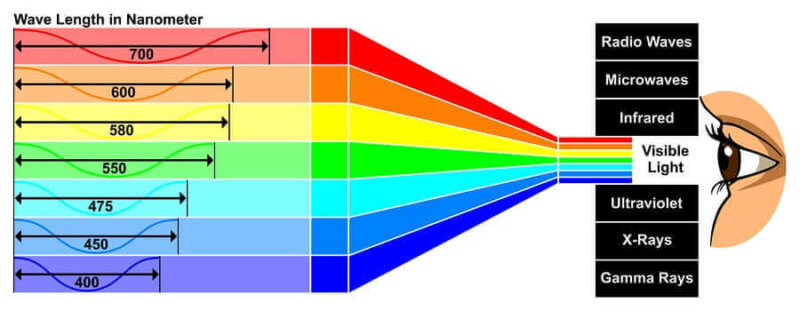
\includegraphics[scale=0.45]{colorimetria3}
            \caption{"Lo spettro visibile"}
        \end{figure}
        \newpage
        \subsubsection{Percezione del colore}
        Il colore nasce dalla luce. La luce che colpisce un oggetto viene parzialmente assorbita a
        seconda del materiale che lo compone. La parte non assorbita viene riflessa e trasmessa ai recettori cromatici
        all’interno dell’occhio umano. Questi ultimi trasformano la luce assorbita in impulsi che
        percorrono le vie nervose fino a raggiungere il cervello, dove vengono interpretati: nasce così
        un’impressione cromatica. Dal punto di vista prettamente biologico il colore si genera pertanto
        nell’occhio dell’osservatore e costituisce un’impressione sensoriale.
        Proprio perché nella percezione del colore vengono coinvolte componenti biologiche, ciascun individuo "percepisce" il colore in modo
        differente. Tale fenomeno può essere ricondotto sia al fatto che non esistono mai due occhi
        uguali tra loro sia al fatto che l’interpretazione del colore varia da individuo ad individuo.
        Perfino la stessa persona può percepire differentemente il colore in momenti diversi ed in base
        allo stato d’animo. È quindi molto complesso definire in maniera oggettiva un colore.

        \begin{figure}[h]
            \centering
            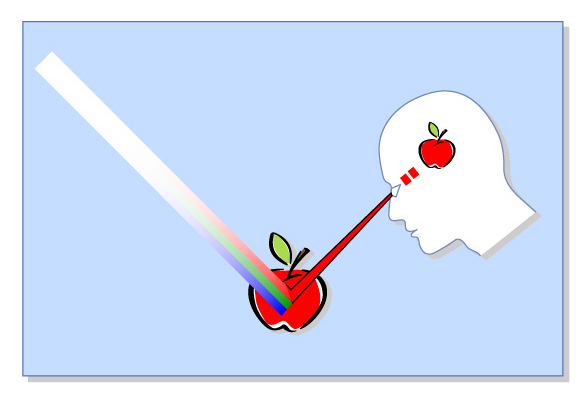
\includegraphics[scale=0.8]{colorimetria1}
            \caption{"Percezione del colore"}
        \end{figure}
        \newpage
        \subsection{Spazio colore}
        Gli spazi colore sono schemi di rappresentazione dei colori. Ognuno di essi si basa su alcuni parametri
        e facendoli variare riesce a rappresentare un numero più o meno grande di colori. Esistono numerosi spazi colore
        che, in base alle loro peculiarità, si prestano meglio ad uno specifico utilizzo piuttosto che ad un altro.
       
        \subsubsection{Modello CIE XYZ}
        Il modello CIE XYZ rappresenta tutti i colori caratterizzati da tre parametri: luminosità, tinta e purezza, rappresentati attraverso un solido. 
        Del solido viene solitamente rappresentata soltanto la sezione secondo il piano XY, in cui X ed Y indicano la cromaticità (tinta e purezza) mentre la luminosità non viene rappresentata.
        \begin{figure}[h]
            \centering
            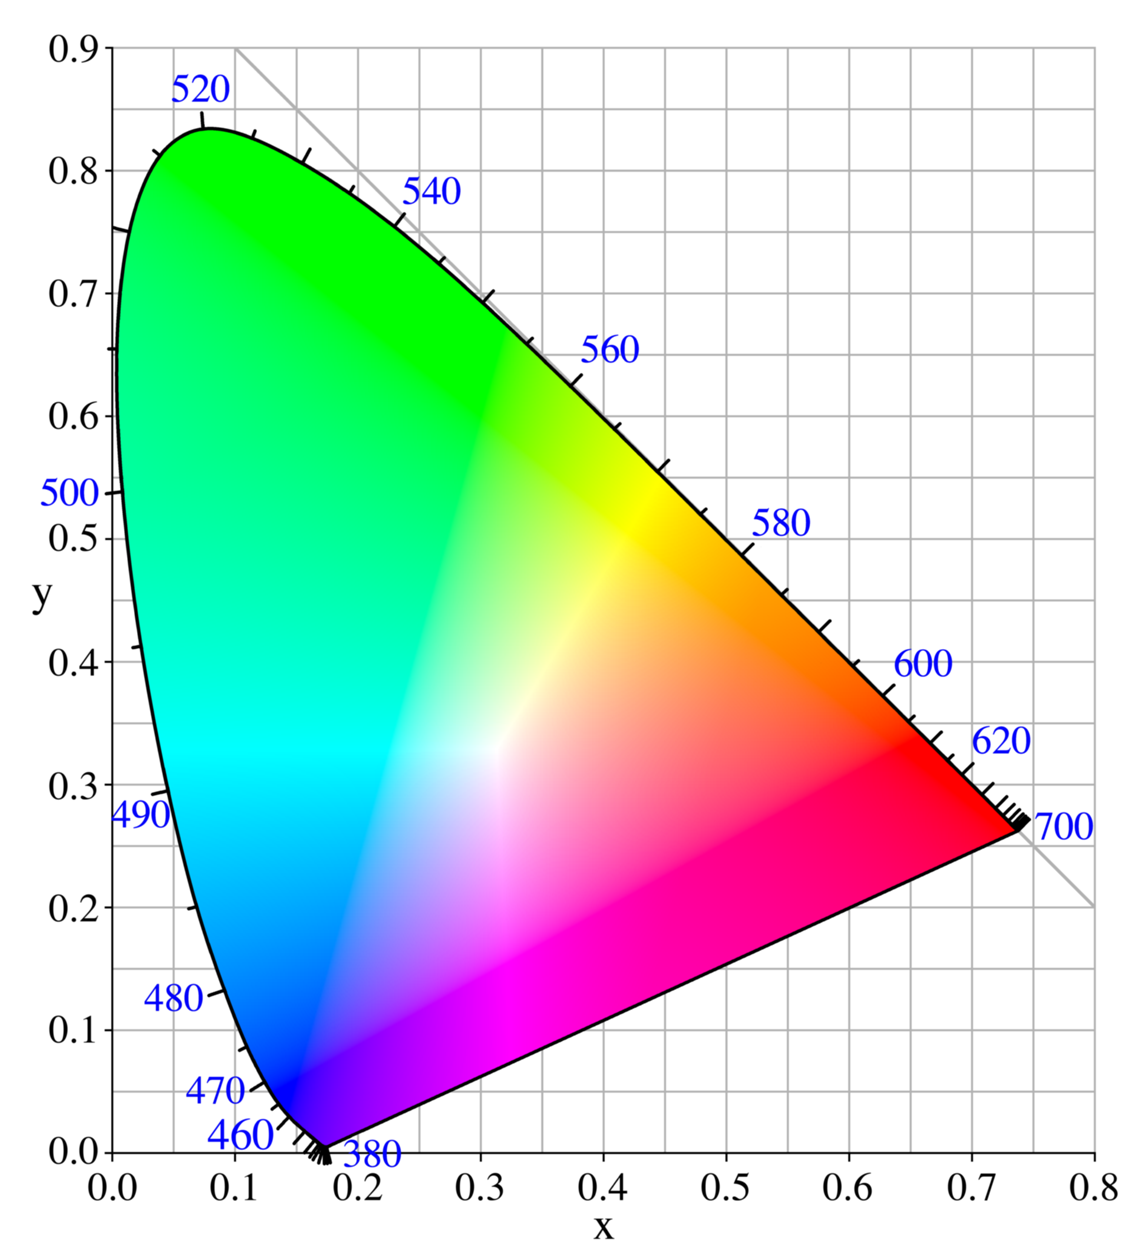
\includegraphics[scale=0.2]{CIEXYZ.png}
            \caption{"Spazio colore CIE XYZ"}
        \end{figure}
        \\Questo spazio colore si basa sui valori di tristimolo, cioè dei parametri che definiscono il modo in cui l'essere umano percepisce i colori. 
        I valori tristimolo di un colore con una distribuzione di potenza spettrale $I(\lambda)$  sono date in termini di un osservatore standard da:
        \\[0.2in]
            $\textbf{X}=\bigint_0^\infty I(\lambda)\,\overline{x}(\lambda)\,d\lambda$;
            $\textbf{Y}=\bigint_0^\infty I(\lambda)\,\overline{y}(\lambda)\,d\lambda$;
            $\textbf{Z}=\bigint_0^\infty I(\lambda)\,\overline{z}(\lambda)\,d\lambda$;
      
        
    
        \newpage

        \subsubsection{Modello CIE L*a*b*}
        Il modello CIE L*a*b*, è un'evoluzione del modello CIE XYZ. È un modello tridimensionale che si sviluppa lungo tre assi ortogonali. Due assi sul piano orizzontale riguardano la cromaticità: l'asse \textbf{a} si estende nel verde (-a) al rosso (+a)
        e l'asse \textbf{b} dal blu (-b) al giallo (+b); un asse verticale riguarda la luminosità o luminanza \textbf{L} che diminuisce dal basso verso l'alto.
        Questo particolare spazio colore include tutti i colori percepibili e quindi anche tutto il gamut degli spazi RGB e CMYK ed è indipendente dal dispositivo che li rappresenta.
        Essendo quindi molto più simile al modo in cui l'essere umano riesce a percepire i colori, questo spazio colore si presta particolarmente bene quando si devono individuare le differenze percettive all'interno di più immagini.

    
        \begin{figure}[h]
            \centering
            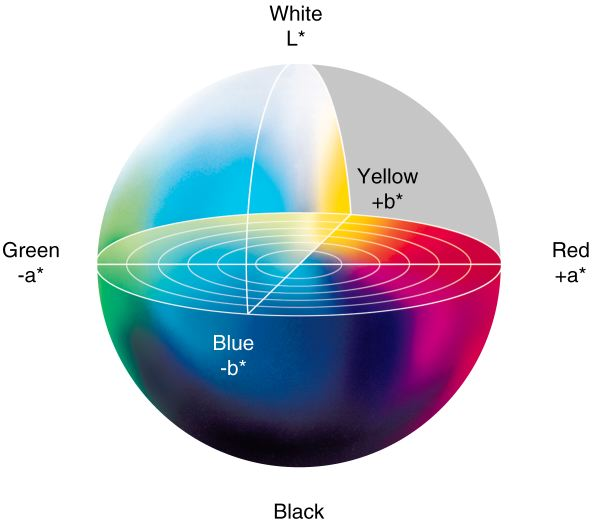
\includegraphics[scale=0.6]{CIELAB.jpg}
            \caption{"Spazio colore CIE L*a*b*"}
        \end{figure}

    \newpage
    \subsection{Risoluzione e compressione}
    La risoluzione di un'immagine corrisponde al numero di pixel per pollice che contiene, indicata con il termine in DPI (punti per pollice). 
    Un maggior numero di dpi si traduce in una maggiore quantità di informazioni e quindi in una migliore qualità dell'immagine. 
    Ovviamente, maggiore è il numero di informazioni che un'immagine contiene, maggiore sarà il peso del file. 
    Per questa ragione sono state sviluppate alcune tecniche di compressione tra cui quella JPEG. Questa tecnica stabilisce due metodi di compressione di base,
    uno basato sull'uso della trasformata discreta del coseno, con compressione di tipo "lossy" e cioè con perdita di informazione, e l'altro sull'uso di un metodo predittivo
    con compressione di tipo lossless, cioè senza perdita di informazione. La perdita di informazioni durante la compressione può compromettere drasticamente la qualità dell'immagine.
    \begin{figure}[h]
        \centering
        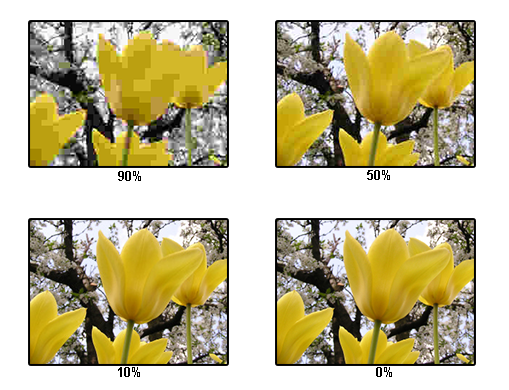
\includegraphics[scale=0.7]{jpeg.png}
        \caption{"Esempio di compressione JPEG"}
    \end{figure}
    \newpage
    \subsubsection{Esempi di risoluzione}
    Ai fini della nostra ricerca, sono state prese in considerazione 5 risoluzioni diverse. Ad ogni risoluzione
    è associata una coppia di valori numerici rappresentativi della larghezza e dell'altezza dell'immagine:
    \begin{itemize}
        \item 4K $\rightarrow$ 3840x2160;
        \item 3K $\rightarrow$ 3000x2000;
        \item 1080p $\rightarrow$ 2048x1080;
        \item 720p $\rightarrow$ 1280x720;
        \item 480p $\rightarrow$ 544x480;
    \end{itemize}
    Il prodotto di questi valori rappresenta il numero di pixel presenti in un'immagine ad una data risoluzione.
    Ad esempio, a 4K avremo $3840*2160 = 8.294.400$, mentre a 480p il numero di pixel sarà $544*480 = 261.120$.
    Quindi un'immagine a 4K userà un numero di pixel decisamente superiore rispetto ad una a 480p e questo le consentirà
    di rappresentare l'immagine con un numero di dettagli superiore e quindi ad una qualità migliore.
    \newpage
    \section {Reti Neurali}
    \subsection {Reti neurali e cervello umano}
    Le reti neurali artificiali sono nate per emulare attività tipiche del
    cervello umano. Risultano quindi molto utili per risolvere problemi di riconoscimento delle immagini o del linguaggio umano.
    Per riuscire ad emulare questi comportamenti ci si è quindi ispirati al funzionamento del cervello umano.
    Nel sistema nervoso esistono miliardi di neuroni. Un
    neurone è formato da un corpo cellulare e da molti prolungamenti
    ramificati, detti dendriti, attraverso i quali il neurone riceve segnali
    elettrici da altri neuroni. Ogni neurone ha anche un prolungamento
    filamentoso chiamato assone. All’estremità l’assone si ramifica formando terminali
    attraverso i quali i segnali elettrici vengono trasmessi ad altre cellule.
    Tra un terminale di un assone e la cellula ricevente esiste uno spazio. I segnali superano questo spazio per
    mezzo di sostanze chimiche dette neurotrasmettitori. Il punto di
    connessione tra terminale e dendrite è detto sinapsi. 
    Un neurone si “attiva”, cioè trasmette un impulso elettrico lungo il suo
    assone quando si verifica una differenza di potenziale elettrico tra l’interno
    e l’esterno della cellula. L’impulso elettrico provoca la liberazione di un
    neurotrasmettitore dai terminali dell’assone, che a loro volta possono influenzare altri neuroni. 
        
    \begin{figure}[h]
        \centering
        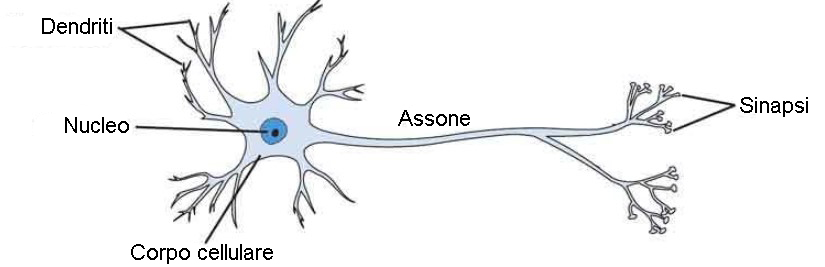
\includegraphics[scale=0.7]{cervello.jpg}
        \caption{"Neurone biologico"}
    \end{figure}

    \subsubsection{Dal neurone biologico a quello artificiale}
    
    Per riprodurre artificialmente il cervello umano occorre realizzare
    una rete di elementi molto semplici in grado di imparare e generalizzare.
    Tipicamente, il neurone artificiale ha molti ingressi ed una sola uscita.
    Per determinate la conducibilità e quindi l'importanza del canale di ingresso, ogni neurone ha associato un peso. 
    L’attivazione del neurone è una funzione della somma pesata degli ingressi.\\[1in]
    Il metodo più usato per addestrare una rete neurale consiste nel presentare
    in ingresso alla rete un insieme di esempi (training set). 
    La risposta fornita dalla rete per ogni esempio viene confrontata con la risposta desiderata, si
    valuta la differenza (errore) fra le due e, in base a tale differenza, si
    aggiustano i pesi cercando di ottenere il risultato desiderato.
    \begin{figure}[h]
        \centering
        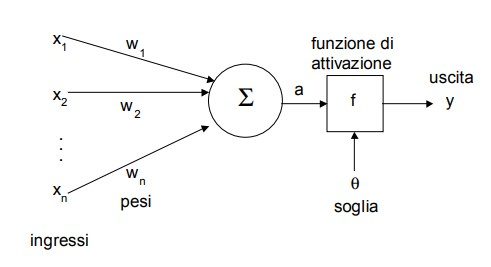
\includegraphics{neurone.jpg}
        \caption{"Modello di neurone"}
    \end{figure}
    \\Abbiamo $n$ canali di ingresso $x_1, …, x_n$, a ciascuno dei quali è associato un peso. 
    I pesi $w_i$ sono numeri reali che riproducono le sinapsi. Se $w_i > 0$, il canale è detto eccitatorio, se $w_i < 0$, il canale è inibitorio. 
    Il valore assoluto di un peso rappresenta la forza della connessione. 
    L’uscita, cioè il segnale con cui il neurone trasmette la sua attività
    all’esterno, è calcolata applicando la funzione di attivazione alla somma
    pesata degli ingressi:
    
    $$y = f(\sum_{i=1}^{n}w_i x_i)$$

    \subsection{Perceptron}
    Un perceptron è una rete neurale ad un singolo livello che si dimostra molto utile nei problemi di classificazione.
    In generale è composto da una serie $x_1, ..., x_n$ di input a cui sono associati dei pesi $w_1, ..., w_n$. 
    Vi è poi una funzione che si occupa di sommare i prodotti dei valori di input e dei rispettivi pesi. 
    Il risultato passa infine per una funzione di attivazione che genera l'output.

    \newpage
    \subsubsection{Addestramento del perceptron}
    Per addestrare un perceptron bisogna realizzare un training set adeguato per il problema che si vuole risolvere. 
    Dopo aver predisposto il dataset è necessario seguire i seguenti passi:
    \begin{enumerate}
        \item si inizializzano i pesi $w_i$ con valori casuali;
        \item si presenta alla rete un ingresso $x_k$ insieme al valore $t_k$ desiderato in uscita;
        \item si calcola la risposta $y_k$ della rete e si aggiornano i pesi mediante la delta rule;
        \item si ripete il ciclo dal passo 2, finché la risposta della rete non risulti soddisfacente.
    \end{enumerate}

    In particolare la delta rule è una regola usata per aggiustare i valori dei pesi di un neurone andando alla ricerca di quelli più adeguati.
    Dati $t$ ed $y$, rispettivamente, l'uscita desiderata e l'uscita neurale, l'errore $\delta$ è dato da:
    $$ \delta = t-y $$
    Fissato un numero reale $\eta$ compreso tra 0 e 1 detto learning rate, la delta rule stabilisce che la variazione del generico peso $\Delta w_i$ è:
    $$ \Delta w_i = \eta \delta x_i $$

    Dopo l’addestramento la rete viene testata controllandone il comportamento su un insieme di dati, detto test set, non utilizzati durante la fase di training. La fase di test ha quindi lo scopo 
    di valutare la capacità di generalizzazione della rete neurale.

  
    \newpage

    \section{Svolgimento}

    \subsection{Creazione del dataset}
    Per poter realizzare la rete è necessario creare un dataset significativo affinché questa possa essere addestrata e testata. 
    Per fare ciò sono state prese in considerazione 40 immagini ad una risoluzione di 4K sulle quali sono state successivamente fatte delle elaborazioni.

    In particolare le elaborazioni sono state:
    \begin{enumerate}
        \item Per ogni immagine nel dataset iniziale è stata generata un'immagine in una risoluzione minore o uguale (4K, 3K, 1080p, 720p, 480p).
        \item Per ogni immagine generata al punto 1 sono stati applicati tre filtri cromatici ciascuno a tre intensità diverse.
    \end{enumerate}
    Tra cui due filtri che coinvolgono indistintamente tutte le zone dell'immagine, ed un filtro che altera solo le zone di una specifica tonalità di colore, in questo caso, quelle del blu.
    Questo procedimento ha così generato 1.200 immagini, utilizzabili per addestrare e testare la rete.
    
    \begin{figure}[h]
        \centering
        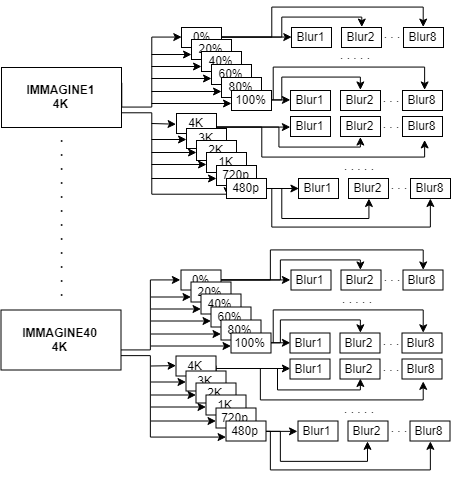
\includegraphics[scale=0.55]{generazione.png}
        \caption{"Generazione del dataset"}
    \end{figure}
    \newpage



    \subsubsection{Codice C++}
    Per ottenere il risultato precedentemente descritto è stato sviluppato un programma in C++ sfruttando la libreria OpenCV.
    Per ogni file nella directory delle immagini vengono generate le immagini a risoluzioni più basse e, per ognuna di queste, vengono applicati i filtri:
    \begin{lstlisting}[language=C++]
        for (dimension resolution : resolutions){
				Size size(resolution.height, resolution.width);
				Mat resizedImage;
				resize(imageOriginal, resizedImage, size);
				string newPath = basePath + "resized/" + resolution.name + "/" + fileName + ".tif";

				if (resolution.name.compare("4K") == 0) 
					copyFile(filePath, newPath);
				else
					imwrite(newPath, resizedImage);
            for (int intensityF1 = 6, double intensityF2 = 1.1, int intensityF3 = 5; intensityF1 <= 56, intensityF2 <= 1.5; intensityF3 <= 15; intensityF1 += 25, intensityF2 += 0.2, intensityF3 += 5) 
            {    
                Mat imageFiltered = applyFilter(newPath, 1, intensityF1);
                string newPathFiltered = basePath + "resized/" + resolution.name + "/filters/" + explode(fileName, '_')[0] + "_B" + to_string(nameCounter) + ".tif";
                imwrite(newPathFiltered, imageFiltered);
                
                imageFiltered = applyFilter(newPath, 2, intensityF2);
                newPathFiltered = basePath + "resized/" + resolution.name + "/filters/" + explode(fileName, '_')[0] + "_B" + to_string(nameCounter+3) + ".tif";
                imwrite(newPathFiltered, imageFiltered);

                imageFiltered = applyFilter(newPath, 3, intensityF3);
                newPathFiltered = basePath + "resized/" + resolution.name + "/filters/" + explode(fileName, '_')[0] + "_B" + to_string(nameCounter+3) + ".tif";
                imwrite(newPathFiltered, imageFiltered);

                nameCounter++;
            }
        }
    \end{lstlisting}

    \newpage
    \subsubsection{Esempi di applicazione dei filtri}
    Di seguito vengono riportati alcuni esempi di immagini generate con il precedente procedimento le cui differenze sono facilmente percepibili ad occhio.
    \begin{figure}[h]
        \centering
        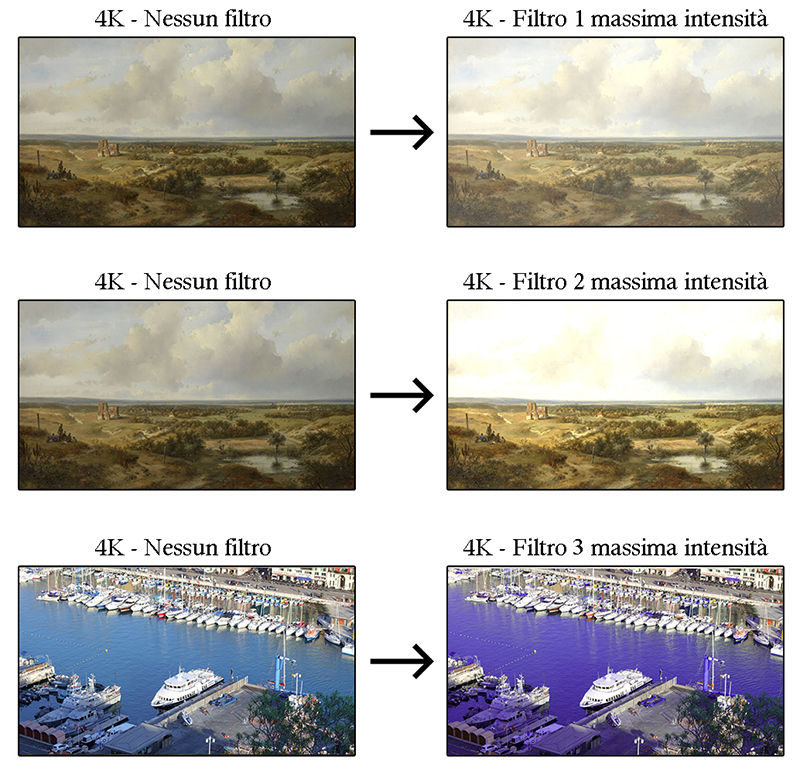
\includegraphics[scale=0.45]{filtri}
        \caption{"Esempi di applicazione dei filtri"}
    \end{figure}


    \newpage
    
    \subsection{Features extraction}
    Per addestrare la rete si è deciso di usare un tipo di addestramento detto "supervisionato". 
    L'addestramento supervisionato è una tecnica di apprendimento automatico che mira a istruire una rete in modo da consentirgli di elaborare automaticamente previsioni sui valori di uscita di un sistema rispetto 
    ad un input sulla base di una serie di esempi ideali, costituiti da coppie di input e di output, che gli vengono inizialmente forniti. L'estrazione delle informazioni dal dataset da fornire come input alla rete, viene detta Features Selection.
    
    \subsubsection{Preparazione degli input e degli output}
    Affinché si possa procedere con l'addestramento, è necessario fornire alla rete dei dati che possa comprendere, in grado di rappresentare
    tutte le immagini da confrontare (input). Dobbiamo inoltre fornire delle valutazioni effettuate da un osservatore umano (output), che indichino la somiglianza tra le varie coppie di immagini da confrontare. 
    Studiando questi dati la rete sarà in grado di emulare il comportamento umano nell'identificazione delle differenze percettive tra due immagini.

    \subsubsection{Estrazione dei dati dalle immagini}
    I dati di input vengono estratti dalle immagini nel nostro dataset. In particolare, questi dati faranno riferimento a zone delle immagini sufficientemente grandi da poter permettere alla rete di comprenderne
    non solo il colore, ma anche la struttura, distinguendone forme e dettagli complessivi. Per fare ciò, tutte le immagini sono
    state suddivise in 9 zone di dimensione uguale e per ognuna di esse sono stati calcolati i valori di media e varianza. Questo procedimento
    viene effettuato per ognuno dei 3 canali (L, a, b).
    Per la media è stata usata la funzione mean() della libreria OpenCV, mentre per la varianza è stata implementata una funzione apposita: 
    \begin{lstlisting}[language=C++]
    double variance(Mat & m, int i, int j, int block_height, int block_width)
    {
        double variance = 0;
        Mat m_tmp = m(Range(i, i + block_height), Range(j, j + block_width)); 
        Mat m_squared(block_height, block_width, CV_64F); 
        
        multiply(m_tmp, m_tmp, m_squared);
        
        double avg = mean(m_tmp)[0]; 	
        double avg_2 = mean(m_squared)[0]; 	
        var = sqrt(avg_2 - avg * avg);
        return variance;
    }
    \end{lstlisting}
    Media e varianza sono tipicamente utilizzati in colorimetria proprio per scopi simili, come ad esempio, nel calcolo dell'SSIM.

    La rete dovrà avere in ingresso la lista dei valori di ogni immagine originale, associata ad ogni sua immagine filtrata. 
    Dopo aver calcolato i valori, questi vengono inseriti in una matrice di dimensione 1800x108, dove 1800 sono il numero di coppie ($Im_i$, $F_j(Im_i, in)$)
    con $Im_i$ immagine $i$-esima, $F_j$ funzione filtro $j$-esima e $in$ intensità del filtro, mentre 108 sono il numero di valori calcolati per ogni coppia.
    
    In particolare, date $X$ ed $Y$ rispettivamente immagine originale e filtrata, $n$ numero di zone su cui sono suddivise le immagini,
    una riga della matrice contiene: 
    \begin{itemize}
        \item ${\mu_x}_i(C)$: media di ogni zona dell'immagine $X$ nei 3 canali;
        \item ${\mu_y}_i(C)$:  media di ogni zona dell'immagine $Y$ nei 3 canali;
        \item ${\sigma^2_x}_i(C)$: varianza di ogni zona dell'immagine $X$ nei 3 canali;
        \item ${\sigma^2_y}_i(C)$: varianza di ogni zona dell'immagine $Y$ nei 3 canali;
    \end{itemize}
    con $i \in (1,n)$ e $C \in (L, a, b)$.
    \\I valori sono quindi: 3 canali * 9 finestre * 4 valori = 108, per riga.
    La matrice di questi valori rappresenterà quindi l'input della nostra rete. 
    \newpage
    \subsubsection{Codice C++}
    Per estrapolare questi valori è stata realizzata la seguente funzione C++:
    \begin{lstlisting}[language=C++]
        for (int k = 0; k < nbBlockPerHeight; k++){
            for (int l = 0; l < nbBlockPerWidth; l++)
            {
                int m = k * block_height;
                int n = l * block_width;
                // Avg values for b-channel
                double avg_ob = mean(img_original[0](Range(k, k + block_height), Range(l, l + block_width)))[0];
                double avg_cb = mean(img_filtered[0](Range(k, k + block_height), Range(l, l + block_width)))[0];
                values.push_back(avg_ob);
                values.push_back(avg_cb);
                // Avg values for a-channel
                double avg_oa = mean(img_original[1](Range(k, k + block_height), Range(l, l + block_width)))[0];
                double avg_ca = mean(img_filtered[1](Range(k, k + block_height), Range(l, l + block_width)))[0];
                values.push_back(avg_oa);
                values.push_back(avg_ca);
                // Avg values for l-channel
                double avg_oL = mean(img_original[2](Range(k, k + block_height), Range(l, l + block_width)))[0];
                double avg_cL = mean(img_filtered[2](Range(k, k + block_height), Range(l, l + block_width)))[0];
                values.push_back(avg_oL);
                values.push_back(avg_cL);
                // Sigma values for b-channel
                double sigma_oa = variance(img_original[2], m, n, block_height, block_width);
                double sigma_ca = variance(img_filtered[2], m, n, block_height, block_width);
                values.push_back(sigma_oa);
                values.push_back(sigma_ca);
                // Sigma values for a-channel
                double sigma_ob = variance(img_original[1], m, n, block_height, block_width);
                double sigma_cb = variance(img_filtered[1], m, n, block_height, block_width);
                values.push_back(sigma_ob);
                values.push_back(sigma_cb);
                // Sigma values for L-channel
                double sigma_oL = variance(img_original[0], m, n, block_height, block_width);
                double sigma_cL = variance(img_filtered[0], m, n, block_height, block_width);
                values.push_back(sigma_oL);
                values.push_back(sigma_cL);
            }
        }
    \end{lstlisting}   
    
    \subsubsection{Preparazione degli output}
    Affinché la rete possa associare i valori rappresentativi di una coppia di immagini da confrontare, 
    ad una valutazione della loro somiglianza, si sono considerati 5 livelli crescenti di affinità: L, ML, MM, MH, H. 
    Sono state quindi analizzate 1800 coppie di immagini (40 immagini * 9 immagini filtrate * 5 risoluzioni), e ad ognuna di queste
    è stato assegnato un livello in questa scala.
    Così come un essere umano guardando una coppia di immagini, riesce ad individuarne le differenze, la rete si comporterà esattamente allo stesso modo ma 
    guardando alle immagini come un insieme di caratteristiche espresse da valori numerici.
    La rete, guardando i valori rappresentativi di una coppia di immagini, cercherà di estrapolare un giudizio basandosi sulla sua esperienza pregressa.
    Questa esperienza gli viene fornita mostrandogli degli esempi, che sono proprio gli output prodotti dal soggetto umano. 
    Quando la rete sarà giunta ad un responso, dovrà comunicare all'esterno il suo risultato. Per farlo utilizzerà i neuroni di output, attivando quello corrispondente al giudizio che ha ottenuto.
    I neuroni di uscita saranno quindi 5 e il valore di uscita della rete sarà:
    \begin{itemize}
        \item {0,0,0,0,1} $\rightarrow$ L 
        \item {0,0,0,1,0} $\rightarrow$ ML
        \item {0,0,1,0,0} $\rightarrow$ MM
        \item {0,1,0,0,0} $\rightarrow$ MH
        \item {1,0,0,0,0} $\rightarrow$ H
    \end{itemize}
    Dove con 1 si indica il neurone attivo e con 0 il neurone non attivo.
    \newpage
    \subsubsection{Esempio di risposta della rete}
    Spieghiamo ciò che si vuole ottenere dalla rete neurale attraverso un esempio. Si considerano due immagini, una originale ed una con applicato il primo filtro alla massima intensità.
    Da esse sono stati estrapolati i dati che le rappresentano, come visto nel paragrafo 4.2.2, che sono poi stati passati in input alla nostra rete.
    Passando attraverso una serie di "livelli nascosti", che la rete crea per effettuare le elaborazioni necessarie all'ottenimento dell'output,
    la rete si accorge che le due immagini sono percettivamente molto diverse tra loro. Procede quindi attivando l'ultimo neurone di uscita.
    \begin{figure}[h]
        \centering
        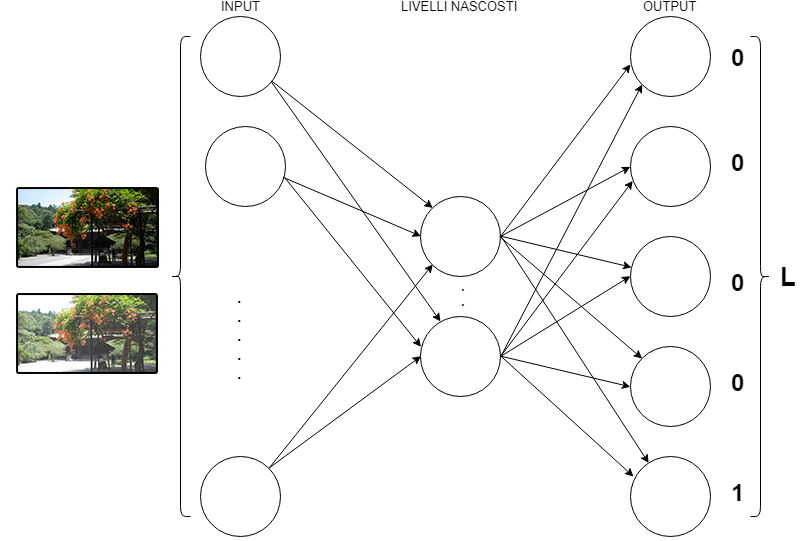
\includegraphics[scale=0.4]{reteneurale}
        \caption{"Esempio di risposta della rete"}
    \end{figure}

    \newpage
    \subsubsection{Esempi di valutazioni da parte dell'osservatore}
    L'osservatore umano, compirà lo stesso procedimento ma assegnando ad ogni coppia di immagini, un valore simbolico, come illustrato nel paragrafo 4.2.4.
    Di seguito vengono riportati alcuni esempi di valutazioni effettuate dall'osservatore umano:
    \begin{figure}[h]
        \centering
        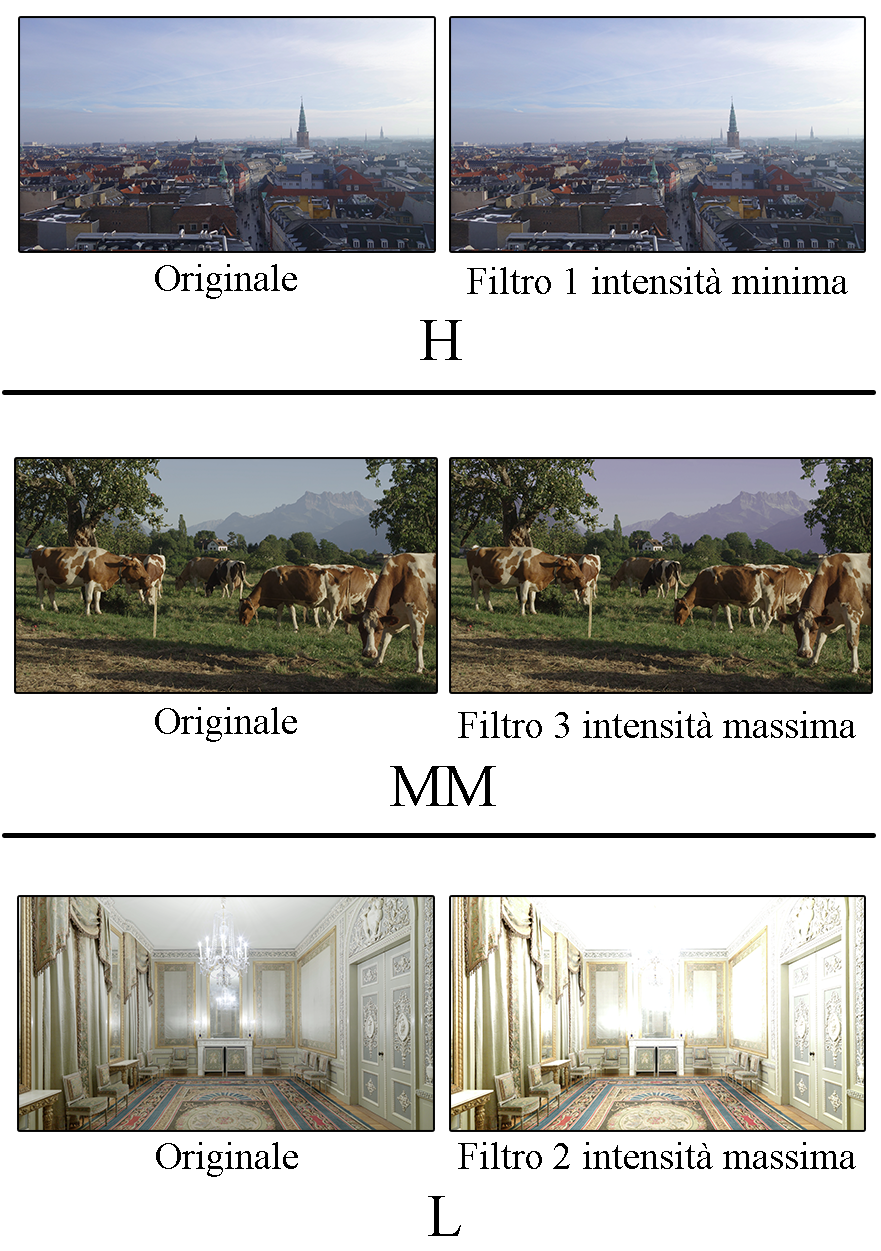
\includegraphics[scale=0.3]{confronto.png}
        \caption{"Esempi di risposta dell'osservatore umano"}
    \end{figure}
    \newpage
    \subsection{Considerazioni preliminari}
    Prima di procedere con l'addestramento della rete, analizziamo i dati ottenuti nei precedenti paragrafi. 
    \subsubsection{Analisi dei giudizi dell'osservatore}
    Prendendo in considerazione tutte le 1800 coppie di immagini originali e filtrate e associandole ai rispettivi giudizi dati
    dall'osservatore umano nel paragrafo 4.2.4, si nota una tendente accentuazione delle differenze cromatiche, al diminuire della risoluzione.
    In particolare, prendendo come esempio il giudizio dato ad una coppia di immagini a 4K e confrontandolo con quello della stessa coppia a risoluzioni inferiori, per tutte le possibili coppie nel dataset,
    si ottengono i seguenti risultati:
    \begin{figure}[h]
        \centering
        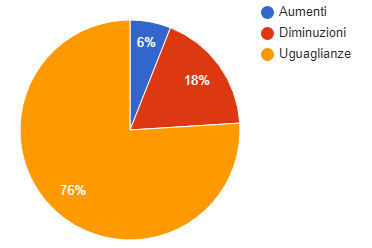
\includegraphics{chart1}
        \caption{"Variazione della percezione umana"}
    \end{figure}
    \\Come si evince dal grafico, all'abbassarsi della risoluzione, le differenze percettive tra le immagini rimangono nella maggioranza dei casi invariate e tendono ad essere accentuate, causando così
    una valutazione più bassa dell'indice di similarità. Ciò accade nel 94\% dei casi presi in considerazione.
    \newpage
    \subsubsection{Calcolo del Lab-SSIM}
    Per avvalorare questa tesi ed evitare che questo comportamento possa essere riconducibile solo alla percezione dell'osservatore umano preso in considerazione, si è deciso
    di effettuare lo stesso procedimento considerando però un indice matematico capace di esprimere le differenze percettive tra due immagini L*a*b*, il Lab-SSIM.
    Questo indice è diverso dall'SSIM tradizionale e consiste nel calcolare, i valori di luminanza dei canali a e b, di contrasto e di struttura del canale L e fare la media tra tutti questi valori.
    \begin{figure}[h]
        \centering
        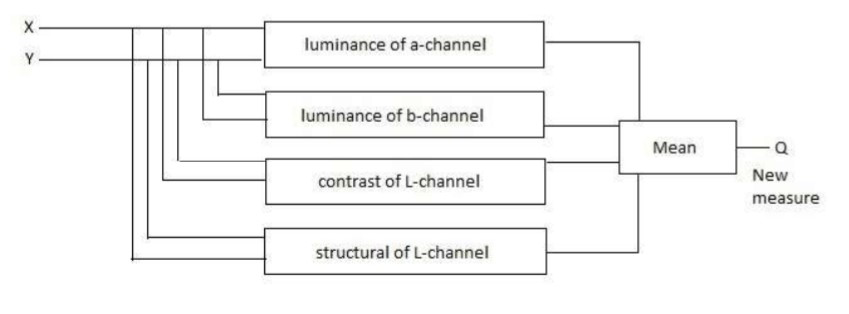
\includegraphics[scale=0.7]{labssim.png}
        \caption{"Lab-SSIM"}
    \end{figure}

    Il Lab-SSIM si basa quindi su tre misurazioni di confronto tra i campioni di $x$ e $y$: luminanza $l$, contrasto $c$ e struttura $s$. Le singole funzioni di confronto sono:
    \begin{enumerate} 
        \item $l(x,y)=\frac{2\mu_x\mu_y + c_1}{\mu^2_x + \mu^2_y + c_1}$
        \item $c(x,y)=\frac{2\sigma_x\sigma_y + c_2}{\sigma^2_x + \sigma^2_y + c_2}$
        \item $s(x,y)=\frac{\sigma_{xy} + c_3}{\sigma_x \sigma_y + c_3}$
    \end{enumerate}
    in cui si hanno:
    \begin{itemize} 
        \item $\mu_x$ e $\mu_y$ la media di $x$ e $y$;
        \item $\sigma_x^2$ e $\sigma_y^2$  la varianza di $x$ e $y$;
        \item $\sigma_{xy}$ la covarianza di $x$ e $y$;
        \item $c_1=(k_1L)^2$, $c_2=(k_2L)^2$ due variabili per stabilizzare la divisione con il denominatore inadatto;
        \item $c_3$ costante pari a $c_2 / 2$.
        \item $k_1=0.01$ e $k_2=0.03$ predefiniti;
   \end{itemize}
   \newpage
    
    \subsubsection{Analisi dei risultati ottenuti con il Lab-SSIM}
    Dopo aver calcolato il Lab-SSIM per tutte le coppie di immagini da confrontare, si passa ad analizzare i risultati, cercando di capire
    se, abbassando la risoluzione, le differenze continuano ad essere visibili. Si fanno quindi le stesse considerazioni del paragrafo 4.3, ma questa volta
    considereremo come giudizio l'indice e non quello dato dall'osservatore umano.
    \begin{figure}[h]
        \centering
        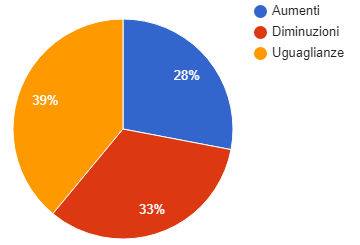
\includegraphics{chart2}
        \caption{"Variazione del Lab-SSIM"}
    \end{figure}
    \\In questo caso, i giudizi rimangono invariati o si abbassano nel 72\% dei casi. La tendenza sembra essere confermata, in quanto le uguaglianze continuano ad essere la maggioranza e le diminuizioni sono superiori agli aumenti, anche se in maniera meno marcata rispetto ai giudizi dell'osservatore umano.
    Da questi risultati si può già intuire che all'abbassarsi della risoluzione, le differenze percettive non solo rimangono percepibili ma tendono addirittura ad accentuarsi.
    \newpage
    \subsection{Addestramento della rete}
    Adesso che siamo in possesso degli input e degli output da fornire alla rete, possiamo passare ad effettuare un primo addestramento.
    Considerando $x$ e $t$ rispettivamente l'insieme delle feature estratte dalle immagini e l'insieme dei giudizi dati dall'osservatore umano, si addestra la rete
    utilizzando il seguente codice Matlab:
    \begin{lstlisting}[language=Matlab]        
        % Funzione di training
        trainFcn = 'trainlm';  
        
        % Creazione della rete
        hiddenLayerSize = 10;
        net = patternnet(hiddenLayerSize, trainFcn);
        
        % Suddivisione del dataset in training, test e validation set
        net.divideFcn = 'dividerand'; 
        net.divideMode = 'sample'; 
        net.divideParam.trainRatio = 70/100;
        net.divideParam.valRatio = 10/100;
        net.divideParam.testRatio = 20/100;
        
        % Funzione per il calcolo delle performance e lista di grafici da generare
        net.performFcn = 'mse';  % mean squared error
        
        net.plotFcns = {'plotperform','plottrainstate','ploterrhist', ...
            'plotconfusion', 'plotroc'};
        
        % Addestramento della rete
        [net,tr] = train(net,x,t);
        
        % Test della rete e performance
        y = net(x);
        e = gsubtract(t,y);
        performance = perform(net,t,y)
        tind = vec2ind(t);
        yind = vec2ind(y);
        percentErrors = sum(tind ~= yind)/numel(tind);

        trainTargets = t .* tr.trainMask{1};
        valTargets = t .* tr.valMask{1};
        testTargets = t .* tr.testMask{1};
        trainPerformance = perform(net,trainTargets,y)
        valPerformance = perform(net,valTargets,y)
        testPerformance = perform(net,testTargets,y)
    \end{lstlisting}
    Il dataset iniziale è stato diviso in 3 parti: Training Set, Validation Set e Test Set. Essi servono rispettivamente per addestrare, validare e testare la rete.
    In particolare, il Training Set serve per far capire alla rete quali risposte deve dare in base agli input che gli vengono forniti, il Validation Set serve per evitare il fenomeno dell'overfitting mentre il Test Set serve per valutarne le performance alla fine dell'addestramento.
    \newpage
    \subsubsection{Valutazione delle prestazioni}
    Una volta completato l'addestramento, per valutarne le prestazioni, analizziamo la matrice di confusione:
    \begin{figure}[h]
        \centering
        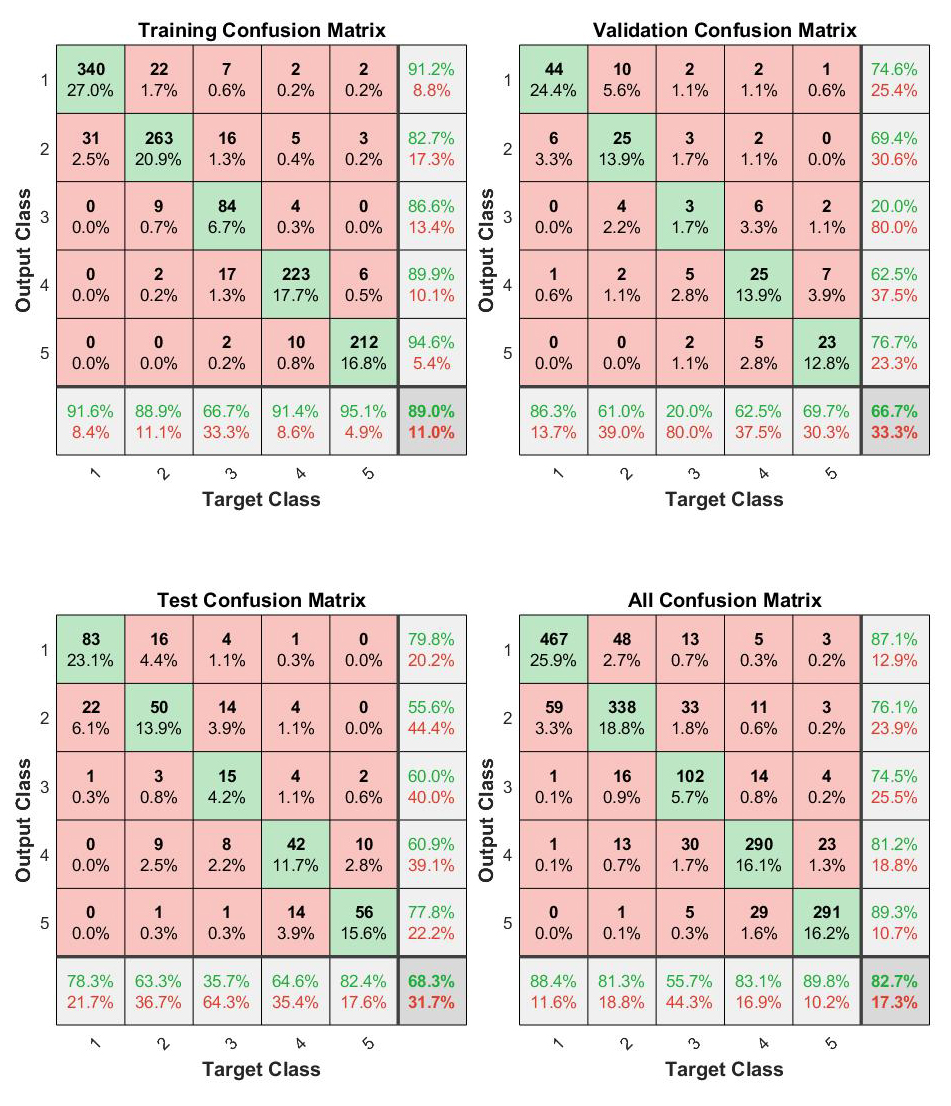
\includegraphics[scale=0.38]{confusion1}
        \caption{"Matrice di confusione"}
    \end{figure}
    \\Ciò che si evince è che l'accuratezza della rete si aggira attorno all'80\%. Questo è già un risultato discreto ma può sicuramente essere migliorato. Idealmente, si vorrebbe ottenere che il 100\% dei giudizi fosse corretto e quindi
    la matrice avrebbe valori soltanto sulla diagonale. In questo caso tuttavia, notiamo una buona precisione sulle valutazioni estreme (H ed L) ma una più scarsa capacità di giudizio delle coppie di immagini con differenze percettive meno marcate.
    Ciò può essere dovuto al fatto che, le reti neurali, necessitano di un numero preciso di dati nel training set affinché possano essere addestrate in maniera corretta.
    Dato $x$ numero di features in input alla rete, e $h$ numero di neuroni presenti nei livelli nascosti, il numero $n$ adeguato di esempi che devono essere presenti nel dataset deve essere:
    $$ n \geq ((x*5)+(h*5))*5 $$

    Nel nostro caso, le features sono l'insieme di varianze e medie calcolate per tutte le coppie (108 features), come descritto dettagliatamente nel paragrafo 4.2.2, mentre i neuroni nascosti sono fissati a 10 per ipotesi.
    Effettuando il calcolo di cui sopra, si ottiene: 
    $$ n \geq ((108*5)+(10*5))*5 = 2.950 $$
    Quindi, per addestrare adeguatamente la nostra rete sarebbero necessari almeno 2.950 esempi di confronti tra coppie di immagini.
    Non disponendo di questi dati, ciò che possiamo fare è effettuare la features selection, cioè l'identificazione delle features maggiormente discriminanti tra le 108 ottenute durante la features extraction.
    Riducendo il numero di features in ingresso alla rete, anche il numero di esempi necessari sarà ridotto, potendo addestrare adeguatamente la rete anche con soli 1.800 confronti.
    \subsubsection{Features selection}
    Durante la features selection, si applica un algoritmo in grado di identificare, tra le varie features estratte durante la features extraction, quelle che contribuiscono maggiormente all'ottenimento del risultato.
    Conoscendo questo dato, è poi facile diminuire il numero di features in ingresso alla rete, andando a selezionare solo quelle che servono veramente alla rete. 
    Per effettuare la features selection si comincia selezionando una feature dal dataset iniziale, essa sarà data in ingresso ad una rete che cercherà di calcolare il risultato di cui noi necessitiamo.
    Si osserva il risultato e si passa alla feature successiva. Dopo aver testato la rete con tutte le features prese singolarmente, si procede testandola con tutte le features prese a coppia. Si va avanti così aggiungendo di volta in volta una nuova feature ai test.
    Questa tipologia di features selection è detta forward. Esiste anche quella backword in cui si parte dall'insieme totale delle features e si procede eliminandone una ad ogni step.
    Alla fine di questo processo, si osservano i risultati della rete nei vari casi e si prendono le features che hanno permesso di ottenere i risultati migliori.
    \newpage
    \section{Test}
    \lipsum[1-3]

    \newpage
    \section{Conclusioni} 
    \lipsum[1-3]

    \newpage
    \section{Ringraziamenti}
    \lipsum[1-3]
    \end{document}
